\documentclass{urticle}
\newcommand{\mys}[1]{\newpage\section*{#1}}
\begin{document}

\begin{center}
{\LARGE \textbf{Исследование коннектомов\\}}
\vspace{1cm}
{\Large Мокров Никита}

{\large Московский Физико-Технический Институт}

{\large Факультет Радиотехники и Кибернетики}

{\large mokrov@frtk.ru}
\end{center}

\section*{Постановка задачи}
Регулярные профилактические осмотры имеют важное значение для современной диагностики ряда заболеваний. Как известно, легче предотвратить болезнь, чем её лечить, поэтому каждому человеку необходимо знать о возможном появлении у него той или иной болезни. Большинство таких заболеваний не поддается полному лечению, но даёт возможность отсрочить момент появления серьезных симптомов.

Исследование структур мозга может помочь в выявлении болезней Альцгеймера и Паркинсона, аутизма и ряда других ментальных заболеваний. Причины этих болезней тесно связаны с генами, влияющими на созревание синаптических связей головного мозга, однако генетика заболеваний сложна. У больных людей отмечают изменения во многих участках мозга, но как именно они развиваются -- неясно.

Формализация представления человеческого мозга в виде взвешенного графа взаимодействия отдельных его участков, дает нам в руки мощный инструментарий для решения широкого спектра задач. В частности, использование машинного обучения, для обработки таких графов отрывают большие перспективы в выявлении вышеупомянутых болезней.

Поэтому возникает формализованная задача классификации (разделение людей на больных и здоровых). Входными данными будем считать граф смежности коннектома\footnote{Для описания структуры мозга будем пользоваться термином <<коннект\'{о}м>>. Он был предложен в 2005 году независимо двумя исследователями Олафом~Спорнсом и Патриком~Хэгмэнном по аналогии с терминами <<ген\'{о}м>> (полное описание всех генов) и <<проте\'{о}м>> (полное описание строения и функций всех белков). Сегодня под словом <<коннект\'{о}м>> понимают полное описание связей в нервной системе того или иного организма.} человека, для которого известно, болен он или здоров, или, что эквивалентно, матрица смежности этого графа.

\mys{Существующий подход к решению поставленной задачи}
На данный момент поставленная задача решается широким кругом лиц из всех стран мира. Исследования ведутся в различных направлениях: применяются как классические, так и новые методы машинного обучения. В данном отчёте исследование основывается на методе улучшения качества классификации путём сочетания различных способов нормировки, описанном в работе \cite{article1}. В данной работе описаны следующие методы нормализации:
\begin{itemize}
	\item Оригинальная нормализация
	\item Бинарная нормализация
	\item Геометрическая нормализация
	\item Топологическая нормализация			
\end{itemize}

С помощью этого подхода можно учесть многие характеристики графа. Основываясь на предложенном методе были получены существенные результаты \cite{article1} в области машинного обучения в нейронауках.
\section*{Альтернативный подход}
В статье \cite{article1} использовались данные здоровых людей и больных аутизмом (UCLA Multimodal Connectivity Database), которые содержат 94 матрицы смежности размера (264, 264) для графов, которые и представляют коннектомы пациентов. 

Это неизбежно ведёт к проблеме обработки большого количества входных признаков. В этой работе было проверено предположение\footnote{предложено Максимом Пановым} о том, что исходные данные сильно зашумлены. К такому заключению приводят следующие доводы. Во-первых, каждая нервная клетка постоянно обновляет связи со смежными с ней нейронами,  а модель строится лишь для определённых момента времени и состояния человека. Во-вторых, формирование массива данных проводится вручную, путём послойного сравнения последовательных участков мозга.

Для решения этой проблемы воспользуемся спектральным разложением матрицы смежности (для симметричной матрицы -- сингулярным разложением):
\begin{equation}
	\label{SVD}
	A = V \Lambda V^{-1}, 
\end{equation} 

где $V$ -- матрица, составленная из собственных векторов матрицы $A$, а $\Lambda$ -- диагональная матрица, составленная из собственных значений матица $A$.

После чего, будем использовать вместо матрицы $A$, матрицу $A'$, полученную отбрасыванием в произведении (\ref{SVD}) множителя $V^{-1}$:
$$ A' = V \Lambda .$$
Теперь, вместо того, чтобы использовать все собственные вектора и значения, отбросим $k$ самых маленьких по модулю собственных значений и соответствующих им собственных подпространств. Таким образом, вместо матрицы размером $(N, N)$, получим матрицу пониженной размерности $(N, N-k)$, сохраняющую основные свойства исходной матрицы.

\mys{Результаты}
Обучив логистическую регрессию на новой матрице для 100 итераций кросс-валидации, мы получим зависимость значения по метрике ROC AUC от параметра $k$, который определяет количество выкинутых собственных значений и собственных векторов:

\begin{figure}[H]
	\centering{
	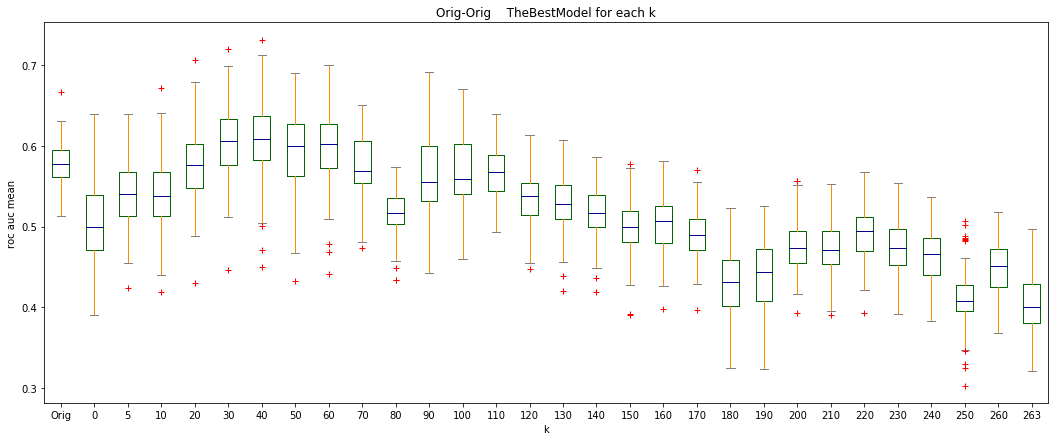
\includegraphics[width=170mm]{1.png}
	}
	\caption{Зависимость ROC AUC mean от $k$ для оригинальной матрицы}
	\label{f1}
\end{figure}

Как правило, лучший подход получается объединением двух или более методов. Поэтому, перед тем как понижать размерность матрицы $A$, можно пробовать по-разному eё нормализовать.
Если воспользоваться бинарной нормировкой, то результат получается гораздо более качественным, прослеживается чёткая зависимость:
\begin{figure}[H]
	\noindent\centering{
	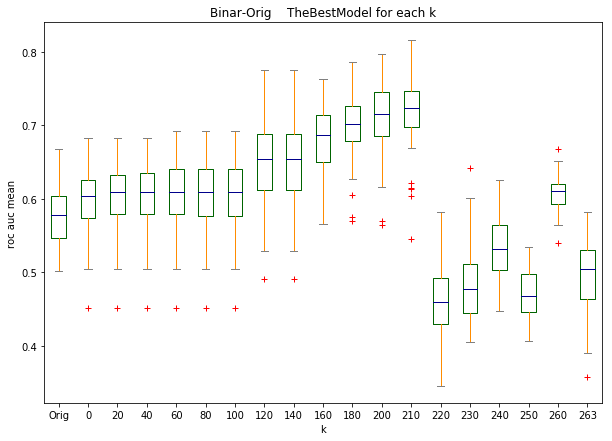
\includegraphics[width=130mm]{2.png}
	}
	\caption{Зависимость ROC AUC mean от $k$ для бинарной матрицы}
	\label{f}
\end{figure}

Данный метод был опробован на других данных (APOE-4), которые содержат пары вида < матрица размером (68, 68), метка класса $\in$ \{болен, не болен\} >. Применим тот же алгоритм на бинарной нормировке для 100 различных итераций:

\begin{figure}[H]
	\noindent\centering{
	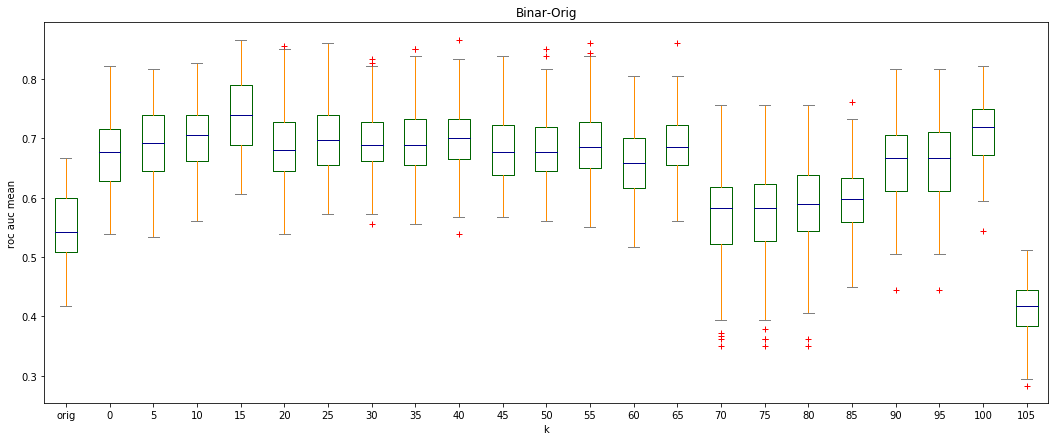
\includegraphics[width=170mm]{3.png}
	}
	\caption{Зависимость ROC AUC mean от $k$ для бинарной матрицы \textbf{парных данных}}
	\label{f3}
\end{figure}

Стоит отметить, что как в работе \cite{article1}, так и в работе \cite{article2}, в которой применялся подход с введением ядра, бинарная нормировка не давала преимущества перед другими. Напротив, в данном исследовании, такой тип предобработки данных был более удачен. С помощью этого метода удалось увеличить результат для обоих данных, в сравнении с использованием оригинальной матрицы, как целевой переменной.

\begin{center}
\begin{tabular}[t]{|c|c|c|}
\hline
	Данные & Результат для $A$ & Результат для $A'$ \\
\hline
	UCLAbaseline & 0.58 & 0.72 \\
\hline
	APOE-4 & 0.54 & 0.73 \\
\hline
\end{tabular}
\end{center}

\mys{Заключение}
В работе было проверено предположение о статистической "шумности" входных данных. Попытка избавиться от неё, попутно уменьшив размерность матрицы смежности и тем самым снизив объём обрабатываемых массивов до разумных значений, привела к успеху: при удачной первоначальной нормировке результат может даже улучшиться по сравнению с исходной матрицей большей размерности.

Естественным образом возникает вопрос о причинах лучшей результативности при использовании бинарной нормировки. Зачастую подобные вопросы не имеют чётких ответов, а результат носит эмпирический характер. В данном конкретном случае можно предположить,  что наибольшее значение имеет не сила взаимодействия между двумя отдельными участками мозга, а сам факт наличия такого взаимодействия, и именно поэтому бинарная нормировка даёт наилучший результат.

\begin{thebibliography}{2}
\bibitem{article1}  Дмитрий Петров, Юлия Додонова, Леонид Жуков и Михаил Беляев. \textit{Boosting Connectome Classification via Combination of Geometric and Topological Normalizations}
\bibitem{article2}  Анвар Курмуков, Юлия Додонова и Леонид Жуков. \textit{Machine Learning Application to Human Brain Network Studies: A Kernel Approach}
\end{thebibliography}

\end{document}
